\clearpage
\section{Operational details}
\label{app:operations}

\subsection{Activation ports}

Table~\ref{tab:ports} fixes each symbol to the tensor consumed by a downstream
product.  Pythia's $a$ and $m$ are distinct LayerNorm outputs on parallel
residual branches.  ``Attention output'' in the diagnostics is after $W_o$ and
is distinct from $z$.

\begin{table}[h]
\centering
\caption{Canonical activation ports.}
\label{tab:ports}
\small
\begin{tabular}{llll}
\toprule
Site & Exact port & Shape & Downstream product \\
\midrule
$a$ & attention-branch norm/gate output & $[B,T,d]$ & fused QKV \\
$m$ & MLP-branch norm/gate output & $[B,T,d]$ & MLP up/$W_1$ \\
$h$ & MLP nonlinearity/gate output & $[B,T,d_f]$ & MLP down/$W_2$ \\
$q,k$ & immediately after partial RoPE & $[B,H,T,d_h]$ & causal QK \\
$v$ & value from fused QKV & $[B,H,T,d_h]$ & causal PV \\
$z$ & concatenated context before $W_o$ & $[B,T,d]$ & attention output/$W_o$ \\
\bottomrule
\end{tabular}
\end{table}

For QK, a coordinate product at valid pair $(i,j)$ is counted zero if
$q_{i,r}=0$ or $k_{j,r}=0$.  For PV, it is counted zero if the causal attention
probability $p_{i,j}=0$ or $v_{j,r}=0$.  Masked future pairs are absent, rather
than credited as zeros.  Projection products use the corresponding activation
and weight operands.  Exact zero means floating-point equality to zero; the
$10^{-3}$ and $10^{-2}$ near-zero diagnostics are separate metrics.

\subsection{Topology-conditioned analytic reach}

\begin{table}[h]
\centering
\caption{Analytic selected-site reach $\Rmax$ for full length-2,048 sequences.
It is not an observed sparsity or speedup.}
\label{tab:ceilings}
\small
\begin{tabular}{lrrr}
\toprule
Topology & Pythia-14M & Pythia-70M & Pythia-410M \\
\midrule
\Afour{} ($a,m,h,z$) & 12.833\% & 37.063\% & 74.776\% \\
\Aseven{} ($a,m,h,q,k,v,z$) & 29.952\% & 49.424\% & 87.245\% \\
\bottomrule
\end{tabular}
\end{table}

The reach numerator credits a selected site to the operation it can null:
$a\rightarrow$QKV, $m\rightarrow W_1$, $h\rightarrow W_2$,
$q$ or $k\rightarrow$QK once, $v\rightarrow$PV and (if all values vanish)
$W_o$, and $z\rightarrow W_o$.  The denominator is exactly that of
Eq.~\ref{eq:rmodel}.  Since measured $\Rmodel$ counts natural zeros everywhere,
it is not required to lie below this selected-site analytic quantity.

\section{Additional quality--opportunity views}

\begin{figure}[H]
  \centering
  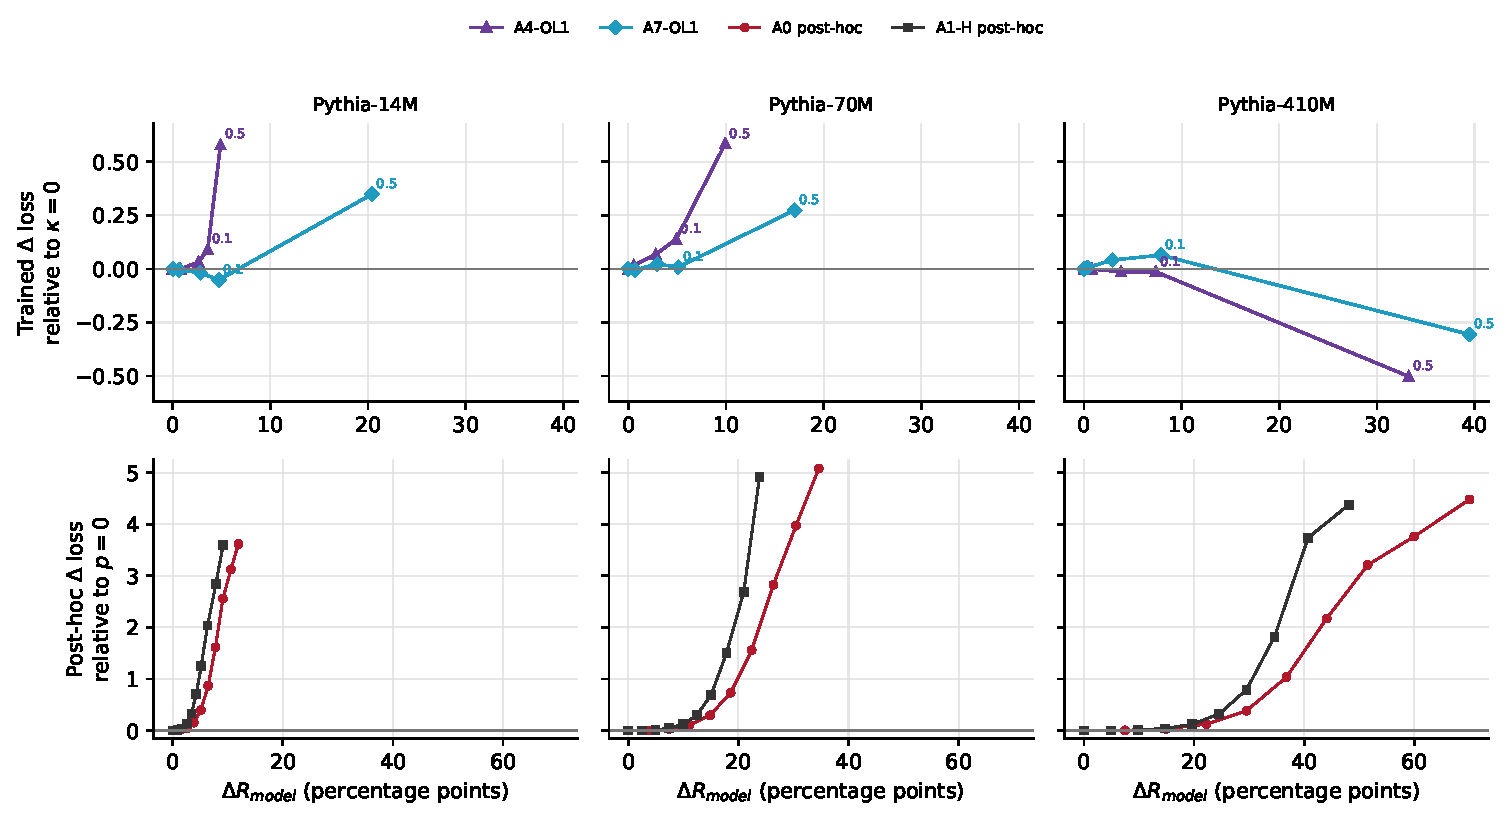
\includegraphics[width=\textwidth]{figures/02-within-scale-deltas.pdf}
  \caption{Within-family change relative to each zero-dose point.  Top:
  trained threshold ladders.  Bottom: evaluation-only clipping paths.  The
  trained 410M direction reverses while both post-hoc families retain positive
  loss cost.}
  \label{fig:deltas}
\end{figure}

\begin{table}[h]
\centering
\caption{Pythia-410M A0 learning-rate screen.  Selection was predeclared on the
mean task loss over boundaries 649--712, not validation loss.}
\label{tab:lr-screen}
\small
\begin{tabular}{lrrr}
\toprule
Peak LR & Late train loss & Validation loss & Selected \\
\midrule
$3\times10^{-4}$ & 4.493717 & 4.547456 & yes \\
$6\times10^{-4}$ & 4.513309 & 4.552068 & no \\
$1\times10^{-3}$ & 6.851160 & 6.786663 & no \\
\bottomrule
\end{tabular}
\end{table}

\section{Training dynamics}

\begin{figure}[H]
  \centering
  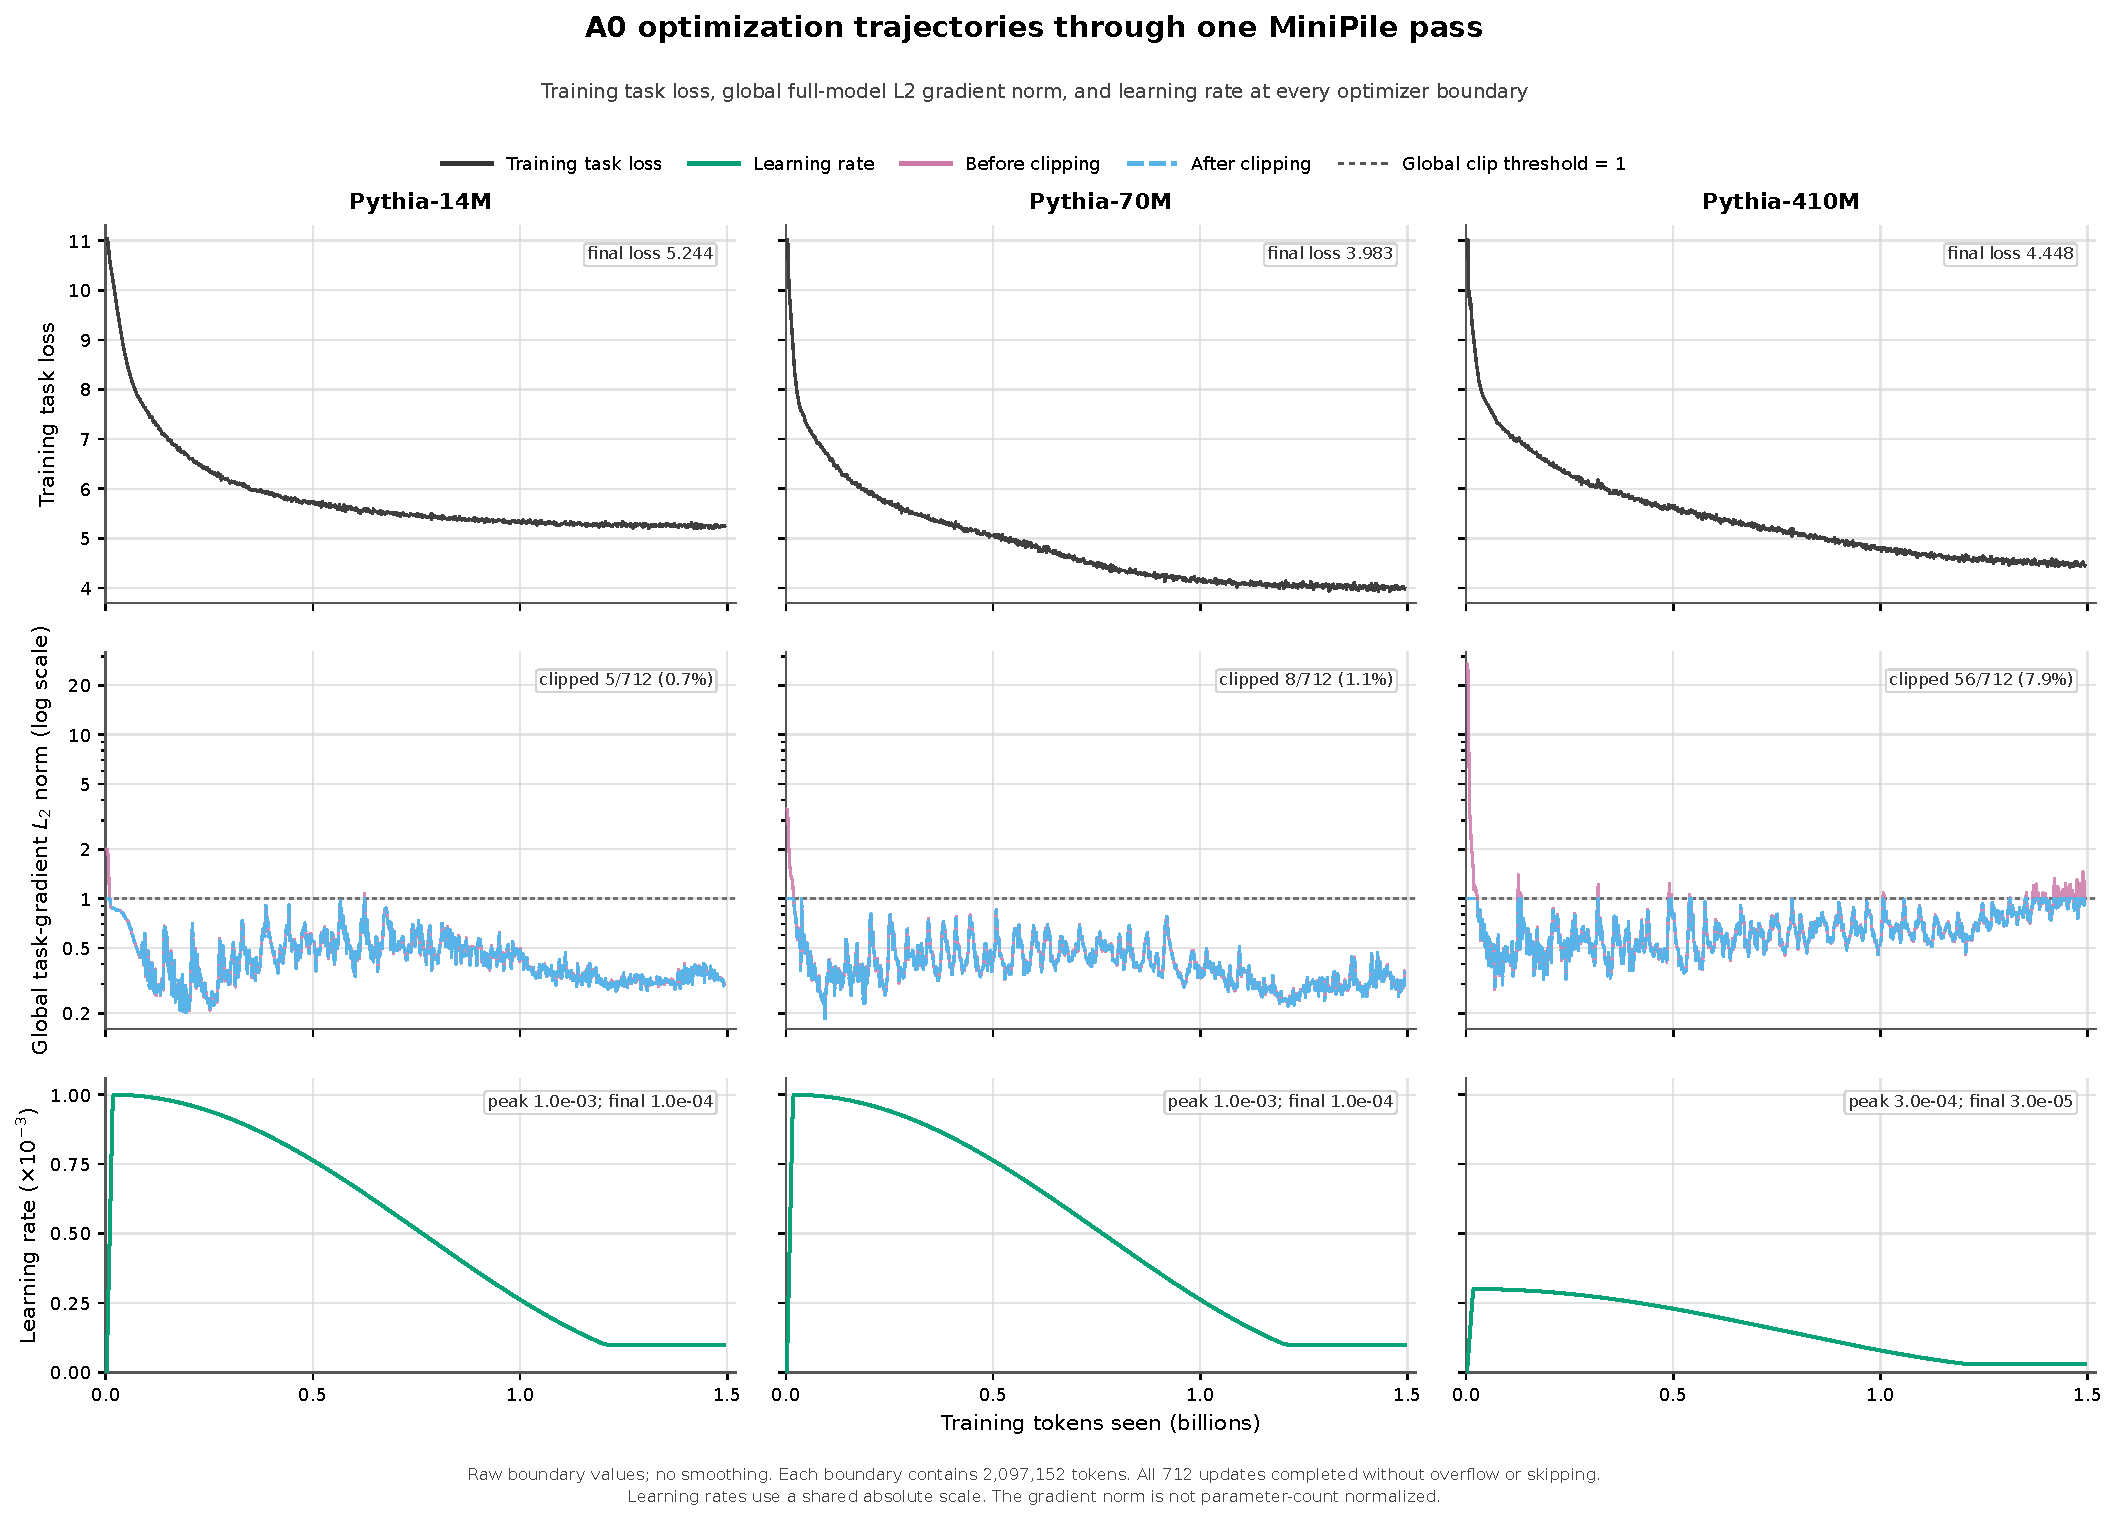
\includegraphics[width=\textwidth]{figures/05-a0-gradient-norm-vs-tokens.pdf}
  \caption{A0 training loss, global task-gradient norm before and after clipping,
  and learning rate over the matched token budget.  These are unnormalized
  global norms, so cross-scale magnitude is descriptive rather than a
  parameter-size-controlled comparison.}
  \label{fig:gradients}
\end{figure}

All streams contain 712 finite boundaries and no skipped update.  A0 has
5/8/56 clipped boundaries and maximum pre-clip norms 2.002/3.513/26.962 at
14M/70M/410M.  The figure is included to expose the executed optimization
regime, not to diagnose the 410M reversal from one scalar trace.

\section{Exploratory sitewise redistribution}

\begin{figure}[H]
  \centering
  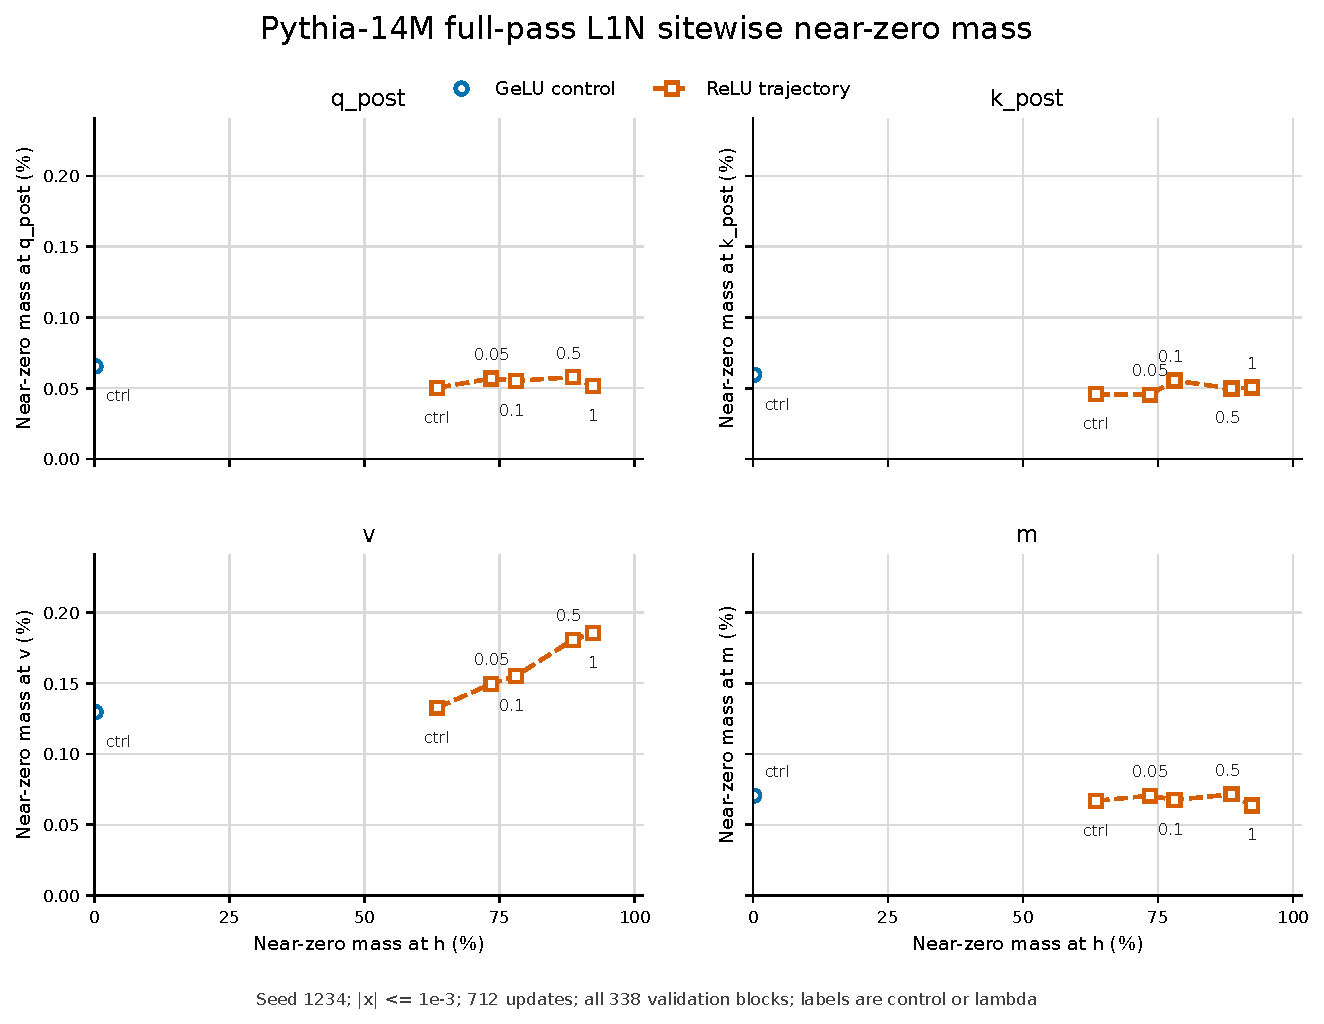
\includegraphics[width=.93\textwidth]{figures/06-spillover-site-grid.pdf}
  \caption{Pooled near-zero mass ($|x|\leq10^{-3}$) at unpressured sites versus
  directly pressured $h$ in a separate Pythia-14M ReLU/naive-$\ell_1$ cohort.
  Lines order pressure dose and are not temporal trajectories.}
  \label{fig:spillover}
\end{figure}

\begin{figure}[H]
  \centering
  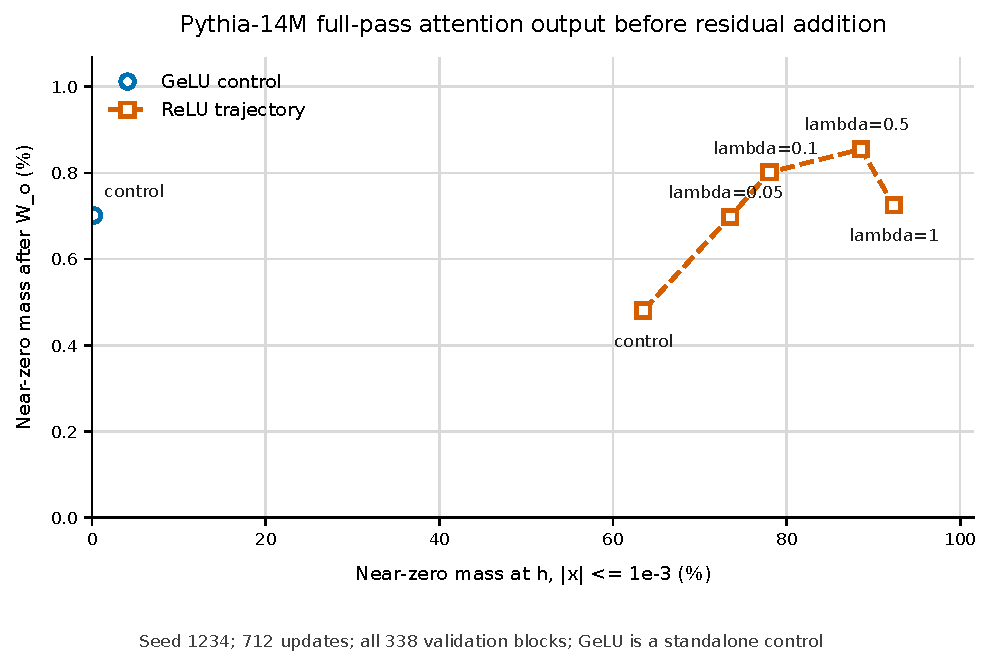
\includegraphics[width=.72\textwidth]{figures/07-attention-output-near-zero.pdf}
  \caption{Near-zero mass after $W_o$ versus at $h$ in the same exploratory
  cohort.  The output response rises through the middle doses and falls at the
  largest pressure.}
  \label{fig:spillover-output}
\end{figure}

All points in Figures~\ref{fig:spillover}--\ref{fig:spillover-output} cover the
same complete validation set.  They use near-zero rather than exact-zero mass
and a different pressure recipe from the main ladder; they support only the
descriptive statement that redistribution is site-specific and non-monotone.

\section{Orthogonal-pressure diagnostic}
\label{app:ol1}

In a matched Pythia-14M A1-H cohort, OL1 minus naive-$\ell_1$ validation loss
was $-0.0081$ and $-0.0061$ at $\lambda=.05$ and $.1$, then $-0.0025$ and
$+0.0188$ at $\lambda=.5$ and $1$.  Exact-zero mass and $\Rmodel$ were nearly matched.
Along naive-$\ell_1$ trajectories, negative raw task--pressure dot products
occurred at 49.2--70.9\% of boundaries as dose increased.  OL1 projected its
own negative Adam-relative interactions to the orthogonal boundary, but this
geometric guarantee did not yield a consistently better endpoint.

\begin{figure}[H]
  \centering
  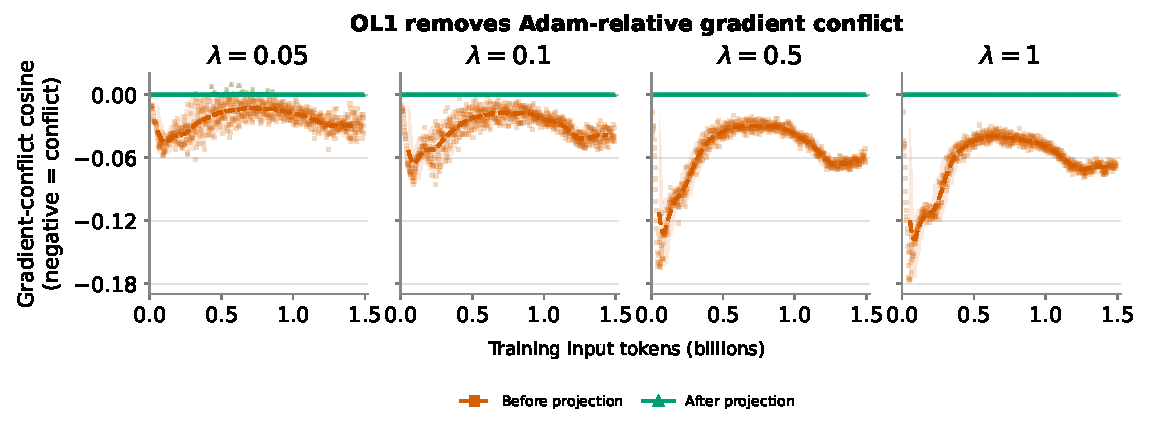
\includegraphics[width=\textwidth]{figures/08-ol1-orthogonalization-trajectories.pdf}
  \caption{OL1 Adam-relative task--pressure interaction before and after the
  operational projection in the separate 14M diagnostic.  Rolling summaries
  describe temporally dependent boundaries, not replicate uncertainty.}
  \label{fig:ol1}
\end{figure}

\section{Reproducibility identities}

The dataset is \texttt{JeanKaddour/minipile} at revision
\begin{quote}\small\texttt{18ad1b0c701eaa0de03d3cecfdd769cbc70ffbd0}.\end{quote}
The tokenizer is \texttt{EleutherAI/pythia-14m-deduped} at revision
\begin{quote}\small\texttt{7386d9a4ae45aef494a6e704910394def3037fc5}.\end{quote}
Encoding adds no special tokens and appends EOS per document.  The training
cache contains 1,491,711,416 tokens and 728,374 complete blocks (tail 1,464);
the validation cache contains 693,668 tokens and 338 complete blocks (tail
1,444).  Their SHA-256 values are:
\par\noindent Training cache:\par
{\scriptsize\noindent\texttt{da82a2ea2e0080c7fd681c7a93b07d3d9ff3d5357a8640895a82d536a1eaf97c}\par}
\noindent Validation cache:\par
{\scriptsize\noindent\texttt{51cd758fda72f14383da30c358a895d0223c0d1d80b31455d2d842c3656d0451}.\par}

The 410M cohort uses 24 layers, $d=1024$, $d_f=4096$, 16 heads, vocabulary
50,304, and 405,334,016 parameters.  Its canonical initialization has parameter
SHA-256
\par{\scriptsize\noindent
\texttt{76217bf2ef13de2377c7750515a559cb71f574c274476e08408a5f7749ea9cff}.\par}
Mixed GPU models were used for this cohort; condition assignment is execution
provenance and not an intended scientific factor.  Each retrieved archive was
hash-verified before cloud teardown.
